\documentclass{article}
\usepackage{graphicx} % Required for inserting images
\usepackage{amsfonts}
\usepackage{amsmath}
\usepackage{float}

\title{Lecture Notes: Introduction to PINN's}
\author{angc2 }
\date{November 2023}

\begin{document}
\maketitle


\section{Motivation}

Suppose we are in a situation in which we are given a sparse data set (which is not exact with some Gaussian noise) which is insufficient to learn our target function. At first glance, it would seem that this is not a good problem with which to conduct machine learning, however, what if we knew a little bit more? Suppose the data we have should obey some physical law, namely, for some domain $\Omega$ (this could be the time-frame we are interested in, a portion of the plane, etc.), we have that $\forall z \in \Omega \subseteq \mathbb{R}^d$ that

\begin{align}
    \mathcal{F}(\textbf{u}(\textbf{z}); \gamma) = \textbf{f}(\textbf{z}).
\end{align}

where $\textbf{z} = [x_1,...,x_{d-t}; t]$ and $\gamma$ is the set of parameters related to the physical system, usually an Ordinary Differential Equation (ODE) or a Partial Differential equation (PDE). It turns out that we can then use this information in order to learn the phenomena by using the above equation to regularize the loss function when we learn the function.

\subsection{PINNs vs Traditional Models}

\subsubsection{When PINNs are Useful Over Traditional Models}

One question that arises is if we have knowledge of the physics of a problem why we wouldn't just use traditional solvers in order to get a solution?  We will now outline the ways in which PINNs are used and when they should be used over traditional models. 

One advantage is that once we have trained our PINNs model, we have effectively trained the model to solve an entire family of equations. Thus, if we were to do another experiment, we would immediately be able to extrapolate a solution from the new data without training the model again. This is in contrast to the way classical solvers work in which we would need to rerun the entire solver for each time we change initial or boundary conditions. Thus, in some situations in which we will want to quickly and efficiently solve numerous ODEs or PDEs which are all members of the same family PINNs are capable of greatly improving the speed of calculating these solutions.

One example application that this feature of PINNs has been beneficial to is in the field of Hemodynamics. This is the field that studies blood flow which is particularly useful for healthcare applications. In a paper by Kissas et al (2020) a PINNs-based method was developed which allows for patient-specific blood flow models which took advantage of the fact that once trained, the PINNs model is capable of accommodating a whole family of solutions. 

One of the obvious cases in which PINNs would be more useful than traditional models are when we do not have full knowledge of the parameters in a given ODE or PDE. An example of this might be that we have some experimental data where we are trying to model the motion of an object which is affected by an unknown coefficient of friction. Using PINNs, we would be able to add this unknown coefficient to the training and thus learn what the coefficient of friction is using our training.

In a paper by Mao et al (2020) PINNs were used to solve inverse problems for the Euler equations. These are equations that are of interest in fluid dynamics, particularly regarding high-speed aerodynamic flows. The authors used the PINNs model to solve inverse problems which could not be solved using traditional approaches in order to use data to determine density, velocity, and pressure parameters.

\subsubsection{When Traditional Models are preferable}

In many cases, there are still reasons why we would use traditional models over PINNs. These might be cases in which we have complete knowledge of all parameters and initial value and boundary value conditions. In these cases, we have very good traditional solvers (Runge-Kutta, Finite-Element, etc.) which can be used for these occasions.

Another case we might prefer the traditional models is that sometimes, training the PINNs model can take a very long time. For instance, the activation functions used, the neural network architecture, learning rate, are all values which can greatly effect the qualitiy of solution which is produced by the PINN and thus can often require lengthy experimentation (as we encountered in our own experiments). Thus, if you are only solving one or a small number of ODEs or PDEs which have readily available traditional solvers, it would probably be advantageous to just use the traditional solver.


\section{What are PINN's}
% \begin{itemize}
%     \item PINNs, or Physically Informed Neural Networks, combine neural networks with physics to solve partial differential equations.
%     \item Many physical systems can be described using PDE's, take for example; Navier-Stokes equations.
%     \item Some of systems exhibit high nonlinearity, involving initial and boundary values, making them computationally demanding
%     \item often limited and noisy data make them a challenging task for other methods 
% \end{itemize}

Now we will discuss what PINNs actually are. PINNs are neural networks which find the solution to a given problem with a physical law of the form of (1). This neural network seeks to learn the target function $\textbf{u}$ with domain $\Omega$ as in (1). Let the final hypothesis be $\hat{\textbf{u}}$ with domain $\Omega$.

These neural networks have a loss function made up of the sum of a data loss and a physical loss. Let us call the physics loss $\mathcal{L}_{\mathcal{F}}$ and the data loss $\mathcal{L}_{\text{data}}$. We define

\begin{align}
    \mathcal{L}_{\text{data}} = \frac{1}{N_d} \sum_{i = 1}^{N_d} \left( \textbf{u}(\textbf{z}_i) - \hat{\textbf{u}}(\textbf{z}_i) \right)^2
\end{align}

where $N_{d}$ is the number of points we use to calculate the data loss and  $\textbf{z}_i \in \Omega$ ($i = 1,2,...,N_{\mathcal F}$) are the points in the domain at which we test the data loss

\begin{align}
    \mathcal{L}_{\mathcal{F}} = \frac{1}{N_{\mathcal F}} \sum_{i = 1}^{N_{\mathcal F}} \left( \mathcal{F}(\hat{\textbf{u}}(\hat{\textbf{z}}_i); \gamma) - \textbf{f}(\hat{\textbf{z}}_i) \right)^2
\end{align}

where $N_{\mathcal F}$ is the number of points we use to calculate the physics loss and  $\hat{\textbf{z}}_i \in \Omega$ ($i = 1,2,...,N_{\mathcal F}$) are the points in the domain at which we test the physics loss. Since we are mainly focused on the applications to ODEs and PDEs the operator $\mathcal F$ may include derivatives, however, utilizing backpropagation it is possible for us to calculate these derivatives for computation. In face, this auto-differentiation feature of neural networks are what give PINNs so much power.

We then have that the problem becomes

$$\theta^* = \text{argmin}_{\theta} (w_{\mathcal{F}} \mathcal{L}_{\mathcal{F}}(\theta) + w_d \mathcal{L}_{\text{data}}(\theta))$$

where $w_{\mathcal{F}}$ and $w_d$ are experimentally determined weights and $\theta$ encompasses the weights within the neural network and possibly some subset of the parameters $\gamma$ if we are solving an inverse problem.

(Sometimes we also add another loss term to include boundary conditions, however, this is not necessary for all PINNs).

\section{How to make a PINN}

\subsection{Architecture}

The first step of making any PINN is to create your neural network. In literature, deep neural networks are often used with many layers and nodes, however, in our experimentation, we were able to get away with shallower networks by increasing the number of neurons in the hidden layers. The main architectures used in most papers are feed-forward networks, convolutional neural networks, and recurrent neural networks. In our experiments we utilized feed-forward networks. In terms of activation functions, most literature use ReLu, Sigmoid, or $\tanh$ activation functions. In our experimentation, we found that the best results came when using the ReLU activation function.

\subsection{Optimization Algorithm}

The most common optimization algorithms used to train PINNs are the Adam, limited-memory Broyden-Fletcher-Goldfarb-Shanno (L-BFGS), and quasi-Newton optimization algorithms. We found in our case that the Adam algorithm (which is an adaptive learning rate algorithm based on stochastic gradient descent) worked the best.

\subsection{Loss Function}

Let us consider how we would construct the loss function for an example. We will consider the case of logistic growth which describes the population of a single species with the only constraint on population growth being the carrying capacity of the environment. The governing differential equation for this differential equation is

$$\frac{dP}{dt} = r P \left(1 - \frac{P}{K} \right)$$

where $P(t)$ is the population of the species as a function of time, $r$ is the growth rate of the species, and $K$ is the carrying capacity of the environment. Now, suppose we have a set of populations $p_i$ where $1 \leq i \leq N_s$ and corresponding times $t_i$ for each population measure. Then, we calculate the data loss using the mean squared loss function by taking our corresponding model's prediction for each time $t_i$ and let each prediction be $\Tilde{p}_i$ and then we get that the data loss is

$$\mathcal{L}_{\text{data}} = \frac{1}{N_s} \sum_{i = 1}^{N_s} (p_i - \Tilde{p}_i)^2.$$

So far, this is the same as if we were training a neural network with the data without regularization. This is where the magic of PINNs comes in. We also know that the population function $P(t)$ should satisfy the differential equation above. Theoretically, we should have for any time $t$ that

$$P'(t) = r P(t) \left( 1 - \frac{P(t)}{K} \right).$$

Using the property of auto-differentiation, we are able to actually compute this for any given $t$ using our model, for example, using \texttt{pytorch}'s \texttt{autograd.grad} function. Therefore, we can take a new grid of the time frame we are interested in and call it $\tau_i$ with $1 \leq i \leq N_p$. Then we can calculate the loss from not satisfying the differential equation given our model's predictions $\hat{p}_i$ for $i \leq i \leq N_p$ as follows

$$\mathcal{L}_{\text{phys}} = \frac{1}{N_p} \sum_{i = 1}^{N_p} \left( \frac{d\hat{p}_i}{dt} \big\lvert_{t = \tau_i} -  r \hat{p}_i \left( 1 - \frac{\hat{p}_i}{K}\right)\right)^2$$

where $ \frac{d\hat{p}_i}{dt} \big\lvert_{t = \tau_i}$ is the derivative we obtain from auto-differentiation. 

To get our loss function we thus have that

$$\mathcal{L} = w_1 \mathcal{L}_{\text{data}} + w_2 \mathcal{L}_{\text{phys}}$$

where $w_1$ and $w_2$ are constants that we have to find experimentally. In our experimentation, we found that letting $w_1 = 1$ and $w_2$ is between $10^{-2}$ and $10^{-4}$ worked well.

% PINN is a multi-layer neural network to calculate differential equation. The input layer takes in a single feature, time (t), which is reshaped to a 2D tensor for compatibility with the linear layer. There are five hidden layers each consisting 256 hidden neurons with the use of activation function after each hidden layer. The output layer will transform the 256 neurons into a result of 2 with Linear function and without activation. The model should intake training data x and y value, and use Adam optimizer.

\section{Properties}

Now we will discuss some of the properties of the solutions generated by PINNs.

\subsection{Error Analysis}

Given that the PINN uses the neural network in order to approximate the solution, it is the neural network and its underlying architecture that determines how low the error can theoretically approximate a solution. So far, there is very little research existing into whether or not a given PINN will actually converge to the true solution of an ODE or PDE. This is an area in which future research will be necessary in order to determine. In its current state, there are cases where PINNs completely fail to train for unknown reasons. While PINNs seem to produce good results in many cases, there are certain problems involving chaotic behavior and multiscale phenomena which often are not possible to solve using PINNs.

\subsection{Continuity}

Given that PINNs are just utilizing a trained neural network to get a solution, these solutions have the property that they are continuous. This means, that unlike traditional solvers there is no need to rerun the entire algorithm if one wants to find a prediction for some point that was not in the original training mesh.

\section{Discuss Our Experiments}

\subsection*{Experiment 1}

In this experiment, we used PINNs to solve the Logistic Growth ODE using the setup described previously. We compare the outputs of the PINNs algorithm with a plain Neural Network with only data loss to see how the two methods perform. We also include each graph the true solution which was computed using scipy's odeint function. In these plots solid red lines represents the true solution, blue x's represent the samples used for training, and the dashed green line represents the predicted curve for the given model

\begin{figure}[H]
    \centering
    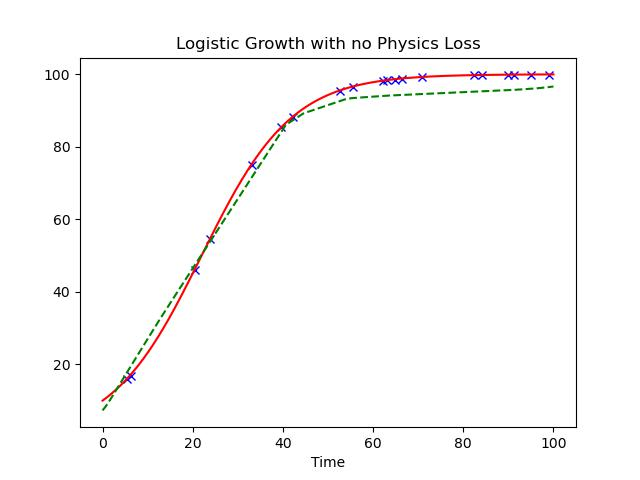
\includegraphics[width=0.5\linewidth]{experiment1_1.png}
    \caption{Experiment 1.1}
\end{figure}

\begin{figure}[H]
    \centering
    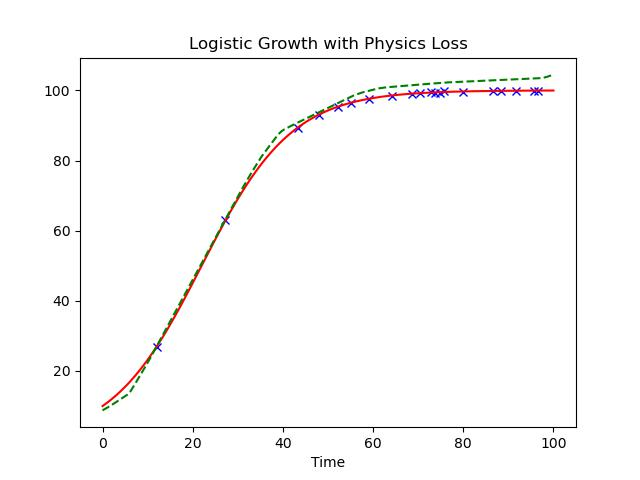
\includegraphics[width=0.5\linewidth]{experiment1_2.png}
    \caption{Experiment 1.2}
\end{figure}

In experiments 1.1 and 1.2, we selected $20$ random points from the true solution with which to train both the normal neural network and the PINNs algorithm both for $700$ epochs. From this, we see that with this number of data points, both methods come up with satisfactory results.

\begin{figure}[H]
    \centering
    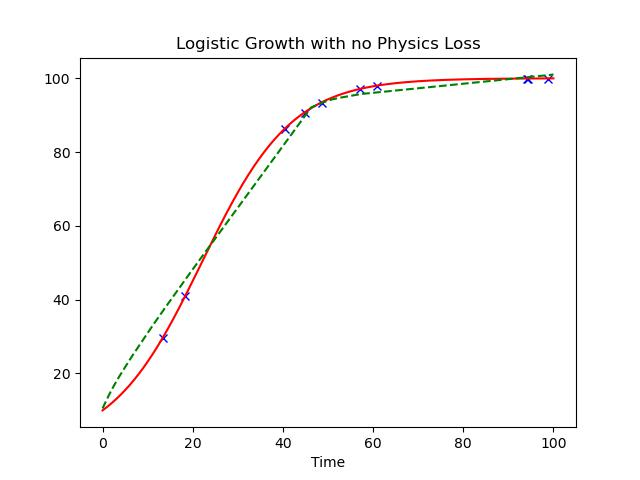
\includegraphics[width=0.5\linewidth]{experiment1_3.png}
    \caption{Experiment 1.3}
\end{figure}

\begin{figure}[H]
    \centering
    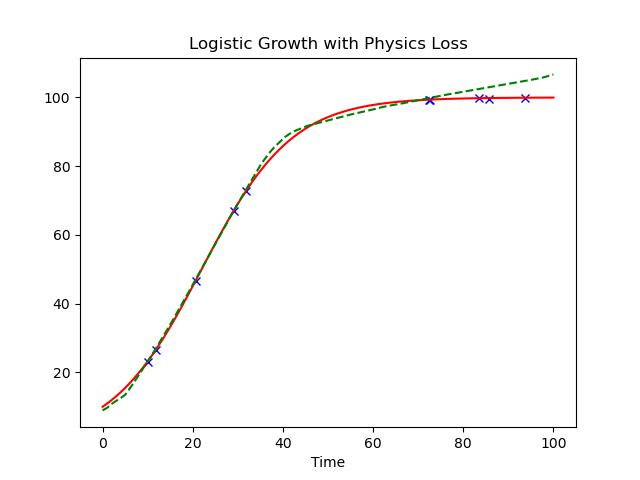
\includegraphics[width=0.5\linewidth]{experiment1_4.png}
    \caption{Experiment 1.4}
\end{figure}

In experiments 1.3 and 1.4, we now only select $10$ random points from the true solution with which to train both algorithms with $700$ epochs. In this experiment, we can see more clearly the effect of the physical loss term in the PINN algorithm. The physical loss term can smooth out the predicted solution to more closely approximate the true solution towards the middle of the curve. 

\begin{figure}[H]
    \centering
    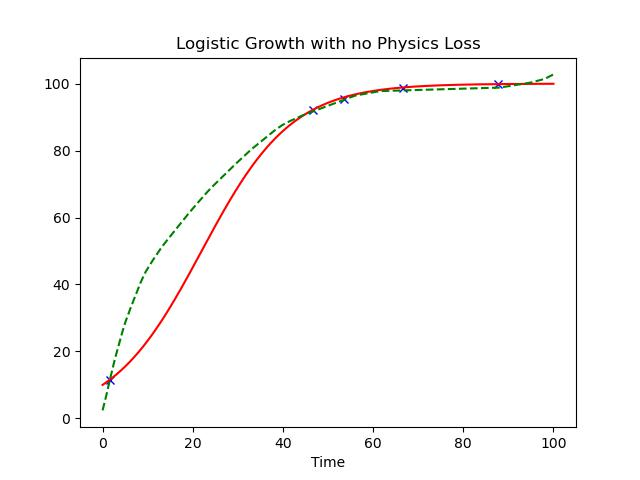
\includegraphics[width=0.5\linewidth]{experiment1_5.png}
    \caption{Experiment 1.5}
\end{figure}

\begin{figure}[H]
    \centering
    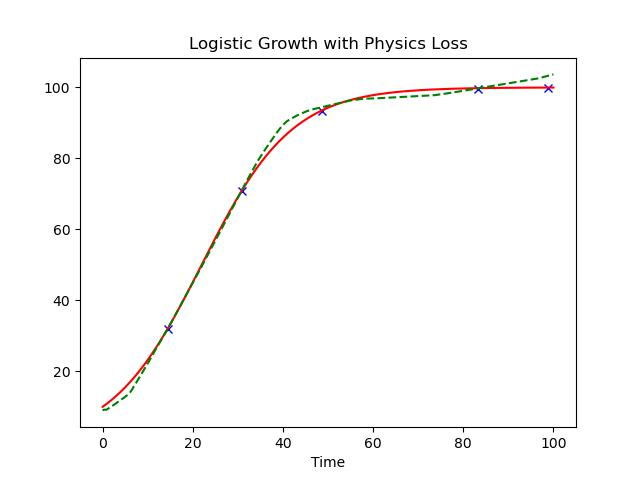
\includegraphics[width=0.5\linewidth]{experiment1_6.png}
    \caption{Experiment 1.6}
\end{figure}

In experiments 1.3 and 1.4, we now only select $10$ random points from the true solution with which to train both algorithms with $700$ epochs. In this experiment, we can see more clearly the effect of the physical loss term in the PINN algorithm. The physical loss term can smooth out the predicted solution to more closely approximate the true solution towards the middle of the curve. 

\begin{figure}[H]
    \centering
    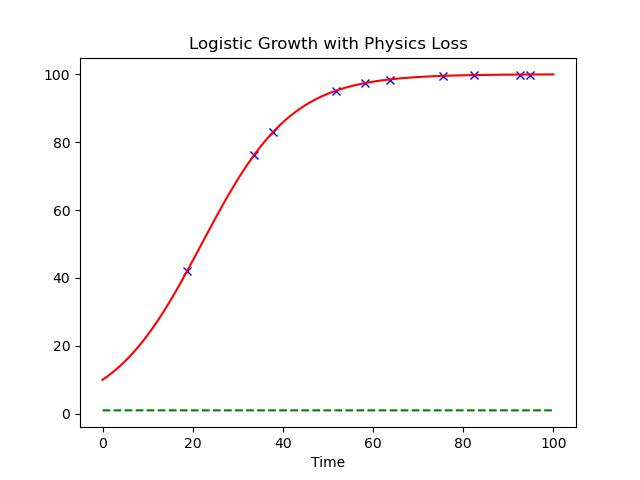
\includegraphics[width=0.5\linewidth]{experiment1_7.png}
    \caption{Experiment 1.7}
\end{figure}

In experiment 1.7 we now show the importance of choosing your activation function. In the previous experiments, we used the ReLU activation function, however, we see that when we switch to the $\tanh$ activation function in this experiment our PINNs model fails to train at all with the same conditions as we had in experiment 1.4 with the same $700$ epochs.

\begin{figure}[H]
    \centering
    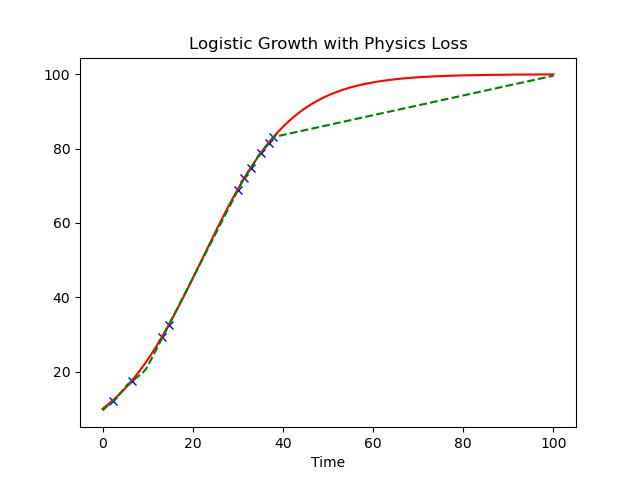
\includegraphics[width=0.5\linewidth]{experiment1_8.png}
    \caption{Experiment 1.8}
\end{figure}

\begin{figure}[H]
    \centering
    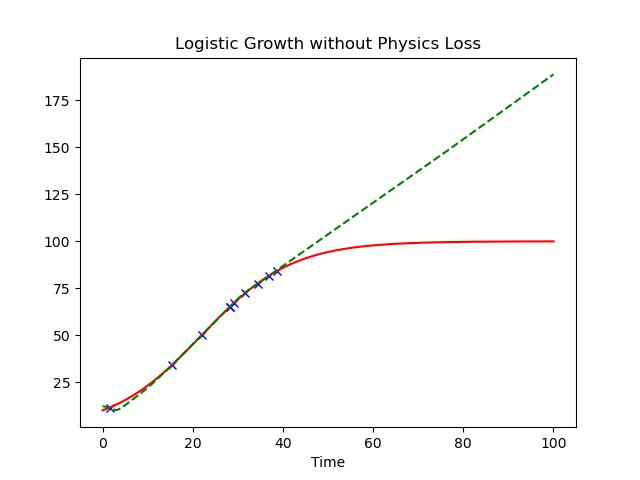
\includegraphics[width=0.5\linewidth]{experiment1_9.png}
    \caption{Experiment 1.9}
\end{figure}

In experiments 1.8 and 1.9 we only took data from the left side of the data. In this case, we only took $10$ random points from the first $40$ units of time. We also run both algorithms with $20000$ epochs. Here we see that without the physics loss, the neural network is not able to determine in experiment 1.8 that after a certain point, the slope should decrease, however, in experiment 1.9 we see that while the PINNs algorithm does not approximate the true solution very well, it still can discern that it should at some point decrease its slope.


In experiments 1.10 and 1.11 we only took data from the left side of the data. In this case, we again took $10$ random points but this time from the first $20$ units of time. We also run both algorithms with $20000$ epochs. Here we see that without the physics loss, the neural network is not able to determine in experiment 1.10 that after a certain point, the slope should decrease, however, in experiment 1.11 we see that while the PINNs algorithm does not approximate the true solution very well, it still can discern that it should at some point decrease its slope.

\subsection*{Experiment 2}

In this experiment, we will be using PINNs to solve the projectile motion differential equation with drag. In this problem, we let the $x$ direction be the horizontal direction and $y$ be the vertical direction. We have that the governing differential equation for $2$D is

$$\frac{d^2 \Vec{s}}{dt^2} = - \mu \left \lVert 
\frac{d \Vec{s}}{dt} \right\rVert_2 \frac{d \Vec{s}}{dt} - \Vec{g}$$

where $\Vec{s}(t)$ is a vector with the $x$ and $y$ components of position, $\mu$ being the coefficient of drag and $g$ being the acceleration of gravity, namely, $g = \begin{bmatrix}
    0\\
    9.8
\end{bmatrix}$.

We then have that our physical loss function then becomes

$$\mathcal{L}_{\mathcal{F}} = \frac{1}{N_{p}}\sum_{i = 1}^{N_{p}} \left\lVert \frac{d^2 \Vec{s}}{dt^2} + \mu \left \lVert 
\frac{d \Vec{s}}{dt} \right\rVert_2 \frac{d \Vec{s}}{dt} + \Vec{g} \right\rVert^2$$

where we calculate the derivatives utilizing pytorch's autograd method.

In this experiment, the solid red line represents the true solution (calculated using odeint), the blue x's represent the points used for data loss and the green lines represent the predicted solution.

\begin{figure}[H]
    \centering
    \includegraphics[width=0.5\linewidth]{experiment2_1.png}
    \caption{Experiment 2.1}
\end{figure}

\begin{figure}[H]
    \centering
    \includegraphics[width=0.5\linewidth]{experiment2_2.png}
    \caption{Experiment 2.2}
\end{figure}

In experiments 2.1 and 2.2 we compare the performance of the neural network without the physics loss and the PINN which utilizes the physics loss. In this problem, we select $10$ data points in the left half of the true solution data. We then run both models for $1500$ epochs. We have that the neural network with only data loss in $2.1$ does not predict a physically possible flight path while this model fits the data, the path predicted crosses over itself and loops back around before going up to infinity. In contrast, the PINN model produces a good approximation of the true solution and produces a believable flight path for the projectile. 

\begin{figure}[H]
    \centering
    \includegraphics[width=0.5\linewidth]{experiment2_3.png}
    \caption{Experiment 2.3}
\end{figure}

\begin{figure}[H]
    \centering
    \includegraphics[width=0.5\linewidth]{experiment2_4.png}
    \caption{Experiment 2.4}
\end{figure}

In experiments 2.3 and 2.4 we now test the ability of PINNs to solve inverse problems while also solving the given ODE. In this experiment, we solve the same problem as in experiments 2.1 and 2.2 but now we do not tell our PINNs model the drag value but add this as a training variable and train for $2500$ epochs. In experiment 2.3 we see what the predicted path is for this problem and we see that even though we removed information, the PINN was still able to make a reasonable approximation of the true solution. In experiment 2.4 we see how the predicted drag depicted as the dashed red line changes by epoch as it approaches the true drag depicted in the blue line. Thus we have now demonstrated PINNs ability to solve inverse problems.

\subsection*{Experiment 3}

Lastly, we do an experiment using the Lotka-Volterra equations which govern the population dynamics of a population of prey and predator species. This differential equation can be represented as

$$\frac{dx}{dt} = \alpha x - \beta x y$$
$$\frac{dy}{dt} = \delta xy - \gamma y$$

where $x(t)$ is the prey population at time $t$, $y(t)$ is the predator population at time $t$, $\alpha$ is the prey birth rate, $\beta$ is the prey death rate, $\delta$ is the predator birth rate, and $\gamma$ is the predator death rate.

We show below what the true solution (using odeint) should look like along with the selected data points.

\begin{figure}[H]
    \centering
    \includegraphics[width=0.5\linewidth]{pred_prey_act.png}
    \caption{True Predator Prey Graph}
\end{figure}

Next, we show the model that our PINN produced

\begin{figure}[H]
    \centering
    \includegraphics[width=0.5\linewidth]{pinn_sol.png}
    \caption{PINN Prediction}
\end{figure}

We have above that the true predator solution is in orange, the true prey solution is in blue, and the data points are shown as blue dots and red x's. We see in the red solid line what the PINN prediction for the predator population is and in the solid green line what the PINN prediction for the prey population is. Our PINN did not succeed in approximating the true solution. Although we tried all sorts of hyperparameters, we were not able to solve this problem using PINNs. This ties into the property of the error convergence of PINNs in that we are not guaranteed that PINNs will converge to the true solution and also demonstrates how difficult it can be to train a PINN.

% \section{Pros}

% PINNs have seen success in many implementations for complicated PDEs from fluid mechanics, hemodynamics, optics, and more. Some particular advantages of PINNs are that once trained, PINNs provide you with a continuous approximation of a function unlike classical finite-difference methods for solving differential equations. This means that once trained, PINNs can essentially tell you predicted value for any value on the domain. We also have that once a PINN is trained on a  Another benefit of PINNs is that from the training data, they can be made to also approximate unknown parameter values. Thus, given a differential equation where one only has partial knowledge of the parameters involved, you can use PINNs to solve the so called 'inverse problem'.

% \section{Cons}

% While PINNs do have some beneficial properties, they are not without their fair share of drawbacks. One of the main drawbacks as with anything involving neural networks are that since neural networks are black-box models, the results often lack interpretability. Also, since we are reformulating differential equations as optimization problems, there is the added possibility that our method will get stuck at a local optimal solution and not converge to the actual (as we will see later in our experimentation). There is also a current lack of PINNs specific optimization algorithms and architecture with many papers using a wide variety of alternatives. Therefore, there is often a large amount of trial and error which needs to take place in order to develop a working PINNs model as opposed to a classical one. This means that PINNs will only be practical to implement in the case of very complicated differential equations which traditional solvers already struggle with.

\section{Future Directions of Research}

One of the most lacking areas in PINN theory is the convergence to the true solution. Do to the black-box nature of neural networks, such research into the accuracy of PINNs has been difficult.

% Another area of interest is why PINNs do not suffer from the 'curse of dimensionality'. One property of PINNs is that they easily scale to higher dimensions as opposed to most classical methods which see exponential increases in computational complexity. 

There also is a lot of practical research to be done into the more specialized optimization algorithms. Currently, the Adam and BFGS algorithms are primarily used in developing PINNs, however, research into algorithms which could help PINNs learn is needed as well as research into the selection of learning rates for optimal results.

\section{References}

Cuomo, S. et al. (no date) Scientific machine learning through physics-informed neural ... - arxiv.org. Available at: https://arxiv.org/pdf/2201.05624.pdf. 

Henderson, I. (2022) Physics informed Neural Networks (pinns): An intuitive guide, Medium. Available at: https://towardsdatascience.com/physics-informed-neural-networks-pinns-an-intuitive-guide-fff138069563. 

Kissas G, Yang Y, Hwuang E, et al (2020) Machine learning in cardiovascular flows modeling: Predicting arterial blood pressure from non-invasive 4D flow MRI data using physics-informed neural networks. Computer Methods in Applied Mechanics and Engineering 358:112,623. https://doi.org/10.1016/j. cma.2019.112623, URL https://www.sciencedirect.com/science/article/pii/ S0045782519305055 

Markidis, S. (2021) The old and the new: Can physics-informed deep-learning replace traditional linear solvers?, Frontiers. Available at:
https://www.frontiersin.org/articles/10.3389/fdata.2021.669097/full. 

Mao Z, Jagtap AD, Karniadakis GE (2020) Physics-informed neural networks for high-speed flows. Computer Methods in Applied Mechanics and Engineering 360:112,789. https://doi.org/10.1016/j.cma.2019.112789, URL https://www.sciencedirect.com/science/article/pii/S0045782519306814

Mishra, S. and Molinaro, R. (2021) Estimates on the generalization error of physics informed Neural Networks (pinns) for approximating pdes, arXiv.org. Available at: https://arxiv.org/abs/2006.16144. 



\end{document}